\section{Training and evaluation of word2vec}
\label{sec:training-and-eval-our-word2vec-impl}
In this section, we will describe how we trained and evaluated our word2vec model. In particular, we will explain the data preprocessing choices we made before training word2vec in \cref{sec:word2vec-data-preprocessing} and details of our implementation of word2vec using the Skip-gram model and negative sampling in \cref{sec:word2vec-impl-specifics}. Finally, we will cover the hyperparameter choices used to train the word2vec model in \cref{sec:word2vec-hyperparameter-choices} and evaluate the performance of the word2vec model using analogy test data sets in \cref{sec:word2vec-model-evaluation}.

\subsection{Data preprocessing}
\label{sec:word2vec-data-preprocessing}
To train a word2vec model, we require a sufficiently large data set and embedding dimensionality to yield good quality word embeddings \cite{mikolov2013b}. In the empirical experiments of \cite{mikolov2013b}, they used an internal data set based on data from Google News. Since this data set was not publicly available, we instead used a Wikipedia dump from \cite{WikimediaDumps} (i.e. a periodic snapshot of the Wikipedia database), and we performed several preprocessing steps before training on it. In particular, we used the \textit{enwiki} (short for English Wikipedia) dump from the 1st of January 2021 (20210101 on the Wikimedia pages). The dump from Wikipedia was first downloaded and parsed using the WikiExtractor tool \cite{Wikiextractor2015}. Furthermore, we created a script using Python to merge and process output files from the WikiExtractor tool into a certain number of text files, such that we could train word2vec at ease. To benefit from parallel reading, we let the number of text files equal the number of CPU cores on our machine.

We then proceeded by processing each Wikipedia article. In particular, we performed the following steps:
\begin{enumerate}
    \item We split each article into a list of sentences using the \path{tokenize.sent_tokenize} function from the \path{nltk} Python package \cite{bird2009natural}.
    \item Then, we preprocessed each sentence individually.
    \begin{enumerate}
        \item We first replaced contractions in each sentence (e.g. I'll $\mapsto$ I will, you'd $\mapsto$ you would, etc.) by using the \path{contractions} Python package \cite{contractions-2016}.
        \item Then we split the sentence into a list of words using the \path{word_tokenize} function from \path{nltk}.
        \begin{enumerate}
            \item We replaced capital letters in words by the corresponding small letters (i.e. lower-case representation).
            \item We removed punctuation from words and created new sub-words for each word delimited by punctuation (e.g. out-of-the-box $\mapsto$ out, of, the, box).
            \item At last, we replaced all numbers (including ordinal numbers) with their textual representation, using the \path{num2words} Python package \cite{num2words2014}. For example, the number 10 was replaced by "ten", and the word "21st" was replaced by "twenty-first".
        \end{enumerate}
    \end{enumerate}
    \item With the new processed sentences, we filtered out sentences that had less than \textbf{min\_word\_count} words in them.
    \item Finally, we appended each sentence to an output text file, separated using the newline character (i.e. \textbackslash n).
\end{enumerate}

After processing the Wikipedia articles into files, we combined common phrases into single tokens. In particular, we followed the word2phrase procedure explained in \cref{sec:learning-word-embeddings-for-phrases}, resulting in tokens consisting of words separated by an underscore, e.g. the phrase "New York" becomes "new\_york". We denoted the threshold hyperparameter from word2phrase as \textbf{threshold-word2phrase}. To create longer phrases of words, e.g. trigrams, four-grams or even five-grams, we repeated the word2phrase multiple times. In particular, we denote the number of repetitions as \textbf{num-epochs-word2phrase}, which we chose as a hyperparameter. Furthermore, for each repetition of word2phrase, the threshold hyperparameter $\delta$ is decreased. \cite{mikolov2013b} did not state how they decreased this threshold, however, but by inspection of the source code of word2vec \cite{Word2vecDemoPhrasesCode}, we observed that they started with a threshold of 200, then decreased it to 100 for the second and final repetition. With this in mind, we introduce a threshold decay hyperparameter, denoted \textbf{threshold-decay-word2phrase}, which tells how much the threshold decreases for each repetition of word2phrase.

\subsection{Implementation specifics}
\label{sec:word2vec-impl-specifics}
To implement the word2vec model, we used Python and TensorFlow \cite{tensorflow2015-whitepaper}. In addition to this, we used the \path{numpy} \cite{2020NumPy-Array} package to work with vectors and matrices more easily. In particular, we implemented the Skip-gram model using negative sampling. To do so, we split our implementation into three main Python classes. The first class is the \path{Tokenizer} class, which is responsible for converting text into word indices in vocabulary (e.g. the word "hello" $\mapsto$ 42). The second class is the \path{Word2vecSGNSModel}, which inherits the \path{tf.keras.Model} class from TensorFlow; we created the model via subclassing, as specified in \cite{TensorflowSubclassing2020}. \path{Word2vecSGNSModel} is the model we used to train our ANN. The third and final main class is \path{Word2vec}. It performs training using the \path{Word2vecSGNSModel} and uses \path{Tokenizer} to convert words into integers.

To load the data into the model, we used the \path{tf.data} API, as introduced in TensorFlow 2. The \path{tf.data} API allows us to create flexible and scalable data generators. As mentioned in \cref{sec:word2vec-data-preprocessing}, we want to train our model on dumps from Wikipedia, i.e. several gigabytes of raw text data, and the \path{tf.data} API allows us to do this quickly and efficiently. In particular, we used the \path{tf.data.TextLineDataset} class to load multiple text files in parallel and set \path{num_parallel_calls} to \path{tf.data.experimental.AUTOTUNE} wherever we could, such that we parallelize the data generation process as much as possible. We also used \path{prefetch} to prepare the data in parallel while training.

We implemented word2phrase using Python. First, we counted the uni- and bigram word occurrences, and using them, we ran the word2phrase procedure as explained in \cref{sec:learning-word-embeddings-for-phrases} by accepting bigrams into the vocabulary if the phrase score (see \cref{eqn:word2phrase-score}) was greater than the set threshold parameter.

By implementing word2vec ourselves, we learned a few things we did not realize after reading the two papers from Mikolov et al. \cite{mikolov2013a, mikolov2013b}:
\begin{itemize}
    \item Training on big data sets (e.g. dumps from Wikipedia) requires an efficient implementation of the data generator. We first attempted to create a data generator that loaded everything into memory, but it became clear to us that this did not scale well when we later wanted to train on bigger data sets.
    \item The quality of the word embeddings depend on the preprocessing of the training data.
    \item That we have two embedding matrices $W$ and $W'$ corresponding to the input and output of the network. At first, we only had a single embedding matrix, for both the input and the output of the network, which led to worse results.
\end{itemize}

\subsection{Hyperparameter choices}
\label{sec:word2vec-hyperparameter-choices}
To train the word2vec model, we based our choices of hyperparameters on the different choices used in models from \cite{mikolov2013a, mikolov2013b}. These hyperparameters can be found in \cref{table:word2vec-hyperparameter-choices}.

\begin{table}[ht]
    \centering
    \begin{tabular}{@{}ll@{}}
    \toprule
    Hyperparameter & Value\\
    \midrule
    \trcolor \textbf{min-word-count} & 5\\
    \textbf{max-vocab-size} & $\infty$ \\
    \trcolor \textbf{batch-size} & 256\\
    \textbf{num-epochs} & 5\\
    \trcolor \textbf{num-epochs-word2phrase} & 2\\
    \textbf{threshold-word2phrase} & 200\\
    \trcolor \textbf{threshold-decay-word2phrase} & 0.5\\
    \textbf{learning-rate} & 0.025\\
    \trcolor \textbf{min-learning-rate} & 0.0000025\\
    \textbf{embedding-dim} & 300\\
    \trcolor \textbf{max-window-size} & 5\\
    \textbf{num-negative-samples} & 5\\
    \trcolor \textbf{sampling-factor} & 0.00001\\
    \textbf{unigram-exponent} & 0.75\\
    \bottomrule
    \end{tabular}
    \caption{Hyperparameters used to train the word2vec model.}
    \label{table:word2vec-hyperparameter-choices}
\end{table}

Similar to \cite{mikolov2013b}, we set the minimum word count to 5 and did not restrict the maximum vocabulary size. In other words, we let the vocabulary include words that occur at least 5 times in the training data.

We set the number of repetitions for word2phrase to 2 and the initial threshold to 200, as \cite{mikolov2013b} did in their experiments. Furthermore, we set the threshold decay to 0.5 (i.e. the threshold is halved for each repetition) to use a similar setup.

Neither \cite{mikolov2013a} nor \cite{mikolov2013b} stated which batch-size they used, but by inspecting the source code of word2vec \cite[line 542]{Word2vecCCode}, we observed that they used 1 as their batch size, i.e. performing a backward pass for every forward pass in the model. We found, however, that setting the batch size to 256 to be a nice fit for our data, leading to good quality vectors and faster training.

Mikolov et al. used 1 to 4 epochs in their experiments \cite{mikolov2013a, mikolov2013b}, and in the source code of word2vec \cite[line 43]{Word2vecCCode}, they default to 5 epochs. For this reason, we set the number of epochs to 5.

We set the initial and minimum learning rate to 0.025 and 0.000025, respectively, as noted in \cite{mikolov2013a} and the source code of word2vec \cite[lines 44 and 398]{Word2vecCCode}.

Furthermore, we set the embedding dimension to 300, the maximal window size to 5, the number of negative samples to 5, the sampling factor to 0.00001 and the unigram exponent to 0.75, similar to experiments from \cite{mikolov2013b}.

Using the preprocessing steps from \cref{sec:word2vec-data-preprocessing} on our data and the hyperparameters from \cref{table:word2vec-hyperparameter-choices}, we get a vocabulary size of $\sim$4.4 million words and corpus size (i.e number of words used from the \textit{enwiki} data set) of $\sim$2.3 billion words.

\subsection{Model evaluation}
\label{sec:word2vec-model-evaluation}
We trained the word2vec model using data preprocessing steps from \cref{sec:word2vec-data-preprocessing} and hyperparameters from \cref{sec:word2vec-hyperparameter-choices}. Following, we will refer to our trained word2vec model as the \textit{SGNS-enwiki} (short for \textbf{S}kip-\textbf{G}ram \textbf{N}egative \textbf{S}ampling-enwiki) model. To show that the trained word embeddings from the SGNS-enwiki model can be used for word analogy tasks, we evaluated the SGNS-enwiki model using analogy test data sets. The goal of performing these tests is to show that the word embeddings of the SGNS-enwiki model are comparable to word embeddings from other published (pre-trained) models in terms of quality.

In particular, we used three analogy test data sets, namely the \textit{Semantic-Syntactic Word Relationship test set} (SSWR), the \textit{Microsoft Research Syntactic Analogies Dataset} (MSR) and the \textit{Phrase Analogy Dataset} (PAD). The SSWR test data set was first introduced in \cite{mikolov2013a}, consists of 8869 semantic and 10675 syntactic questions and is widely used as a test data set. The MSR data set was first introduced in \cite{mikolov-etal-2013-linguistic} and consists of 8000 analogy questions. To evaluate word embedding models trained on phrases (e.g. "New York Times"), \cite{mikolov2013b} introduced the PAD. PAD consists of 3218 analogy questions. It should be noted, however, that there are other common test data sets as well, such as the Bigger analogy test set (BATS) from \cite{gladkova-etal-2016-analogy}.

We compared the results from the evaluation of the SGNS-enwiki model to models from \cite{mikolov2013a, mikolov2013b, mikolov-etal-2013-linguistic, bojanowski2017enriching} in \cref{table:word2vec-eval-sswr,table:word2vec-eval-msr,table:word2vec-eval-pad}. In particular, we compared to the Skip-gram models from \cite[Table 3]{mikolov2013a} and \cite[Table 6]{mikolov2013a} (denoted \textit{SG 300} and \textit{SG 1000} respectively), the \textit{NEG-15} model from \cite[Table 1 and 3]{mikolov2013b}, the \textit{RNN-1600} model from \cite[Table 2]{mikolov-etal-2013-linguistic}, the \textit{GloVe 300 42B} model from \cite[Table 2]{pennington2014glove}, and the \textit{fastText} model from \cite[Table 2]{bojanowski2017enriching}. In \cref{table:word2vec-eval-sswr,table:word2vec-eval-msr,table:word2vec-eval-pad}, a dash (--) denotes that the model has not been evaluated on the particular subset/data set, and \textbf{bold} values indicate the best value. Values represent accuracies and are in percentages.
\begin{table}[H]
    \centering
    \begin{tabular}{@{}cccc@{}}
    \toprule
    & \multicolumn{3}{c}{SSWR} \\ \cmidrule(l){2-4}
    \multirow{-2}{*}{Model} & Semantic & Syntactic & Average \\ \midrule
    \trcolor
    SG 300 & 55 & 59 & 57 \\
    SG 1000 & 66.1 & 65.1 & 65.6 \\
    \trcolor
    NEG-15 & 61 & 61 & 61 \\
    RNN-1600 & -- & -- & -- \\
    \trcolor
    GloVe 300 42B & \textbf{81.9} & 69.3 & 75.0 \\
    fastText & 77.8 & \textbf{74.9} & \textbf{76} \\
    \trcolor
    SGNS-enwiki & 65.8 & 67.3 & 66.6 \\
    \bottomrule
    \end{tabular}
    \caption{Comparison of empirical results of word embedding models evaluated using the SSWR word analogy test data set.}
    \label{table:word2vec-eval-sswr}
\end{table}
\begin{table}[H]
     \centering
    \begin{tabular}{@{}ccccc@{}}
    \toprule
    & \multicolumn{4}{c}{MSR} \\
    \cmidrule(l){2-5} 
    \multirow{-2}{*}{Model} & Adjectives & Nouns & Verbs & Average \\
    \midrule
    \trcolor
    SG 300 & -- & -- & -- & \textbf{56} \\
    SG 1000 & -- & -- & -- & -- \\
    \trcolor
    NEG-15 & -- & -- & -- & -- \\
    RNN-1600 & 23.9 & 29.2 & \textbf{62.2} & 39.6 \\
    \trcolor
    GloVe 300 42B & -- & -- & -- & -- \\
    fastText & -- & -- & -- & -- \\
    \trcolor
    SGNS-enwiki & \textbf{43.1} & \textbf{62.5} & 59.1 & 54.9 \\
    \bottomrule
    \end{tabular}
    \caption{Comparison of empirical results of word embedding models evaluated using the MSR word analogy test data set.}
    \label{table:word2vec-eval-msr}
\end{table}
\begin{table}[H]
    \centering
    \begin{tabular}{@{}cc@{}}
    \toprule
    & PAD \\
    \cmidrule(l){2-2}
    \multirow{-2}{*}{Model} & Average \\
    \midrule
    \trcolor
    SG 300 & -- \\
    SG 1000 & -- \\
    \trcolor
    NEG-15 & 42 \\
    RNN-1600 & -- \\
    \trcolor
    GloVe 300 42B & -- \\
    fastText & -- \\
    \trcolor
    SGNS-enwiki & \textbf{53.7} \\
    \bottomrule
    \end{tabular}
    \caption{Comparison of empirical results of word embedding models evaluated using the PAD word analogy test data set.}
    \label{table:word2vec-eval-pad}
\end{table}

In \cref{table:word2vec-eval-sswr}, we see that the SGNS-enwiki model is fairly competitive in terms of accuracy on the SSWR analogy test data set. The fastText model, however, is the most accurate model on this test data set. In particular, the fastText model is approximately 10\% more accurate on average than the SGNS-enwiki model. The same story goes for the results from the MSR test data set, we see in \cref{table:word2vec-eval-msr}, where the SGNS-enwiki model performs pretty well, falling short for the SG 300 on average. Finally, in \cref{table:word2vec-eval-pad} we see that the SGNS-enwiki model outperforms the NEG-15 model. We note that we had a lot of missing data for this evaluation, as all models had not been evaluated for every (subset of the) test data set. This evaluation, however, indicates that the SGNS-enwiki model understands syntactic and semantic relationships between words.

To gain further insight into how the vector representations learned by the SGNS-enwiki model are, we inspected the nearest neighbours of words. In \cref{table:word2vec-nearest-neighbours-words} we show a sample of such comparison, using the 5 nearest neighbouring words (also some phrases) for each query word. We used cosine similarity to find the neighbouring words, excluding the query word from the search. In \cref{table:word2vec-nearest-neighbours-words}, we see the ability of the SGNS-enwiki model to identify related words to the query word.
\begin{table}[H]
    \centering
    \begin{tabular}{@{}ll@{}}
    \toprule
    Query word & Neighbouring words \\ \midrule
    \trcolor
    Apple        & Apple Inc., Blackberry, Apple computer, OneScanner, released Xsan \\
    Phone      & Phones, mobile phone, cell phone, cellphone, phone calls \\
    \trcolor
    Water   & Fresh water, drinking water, water pumped, salinated, untreated water \\
    Sunny      & Windy, dry sunny, warm sunny, cool, Lee Hany Lee \\
    \trcolor
    Book      & Books, book entitled, Tarcher Penguin, author, foreword \\ \bottomrule
    \end{tabular}
    \caption{The five nearest neighbouring words of some query words. We use cosine similarity and word embeddings of the SGNS-enwiki model.}
    \label{table:word2vec-nearest-neighbours-words}
\end{table}

We visualize the ability of the SGNS-enwiki model to identify underlying concepts of the language and relationships between them in \cref{fig:sgns-enwiki-word-to-word-relations-pca-2d}, using a 2-dimensional PCA (\cref{sec:id-estimation-lpca}) embedding of words representing countries/capitals and comparative adjectives (e.g. good $\rightarrow$ better $\rightarrow$ best). We used PCA instead of UMAP here as there were few points, and PCA typically works better than UMAP in such cases. In \cref{fig:sgns-enwiki-word-to-word-relations-pca-2d}, we see that the SGNS-enwiki models understand what capital means and how comparative adjectives behave. In addition to this, we also observe some clustering occurring in both plots. In particular, we observe that Scandinavian countries and capitals are more clustered to the top of \cref{fig:sgns-enwiki-word-to-word-relations-pca-2d} (a), and words related to temperatures are more clustered to the right of \cref{fig:sgns-enwiki-word-to-word-relations-pca-2d} (b).
\begin{figure}[H]
   \centering
   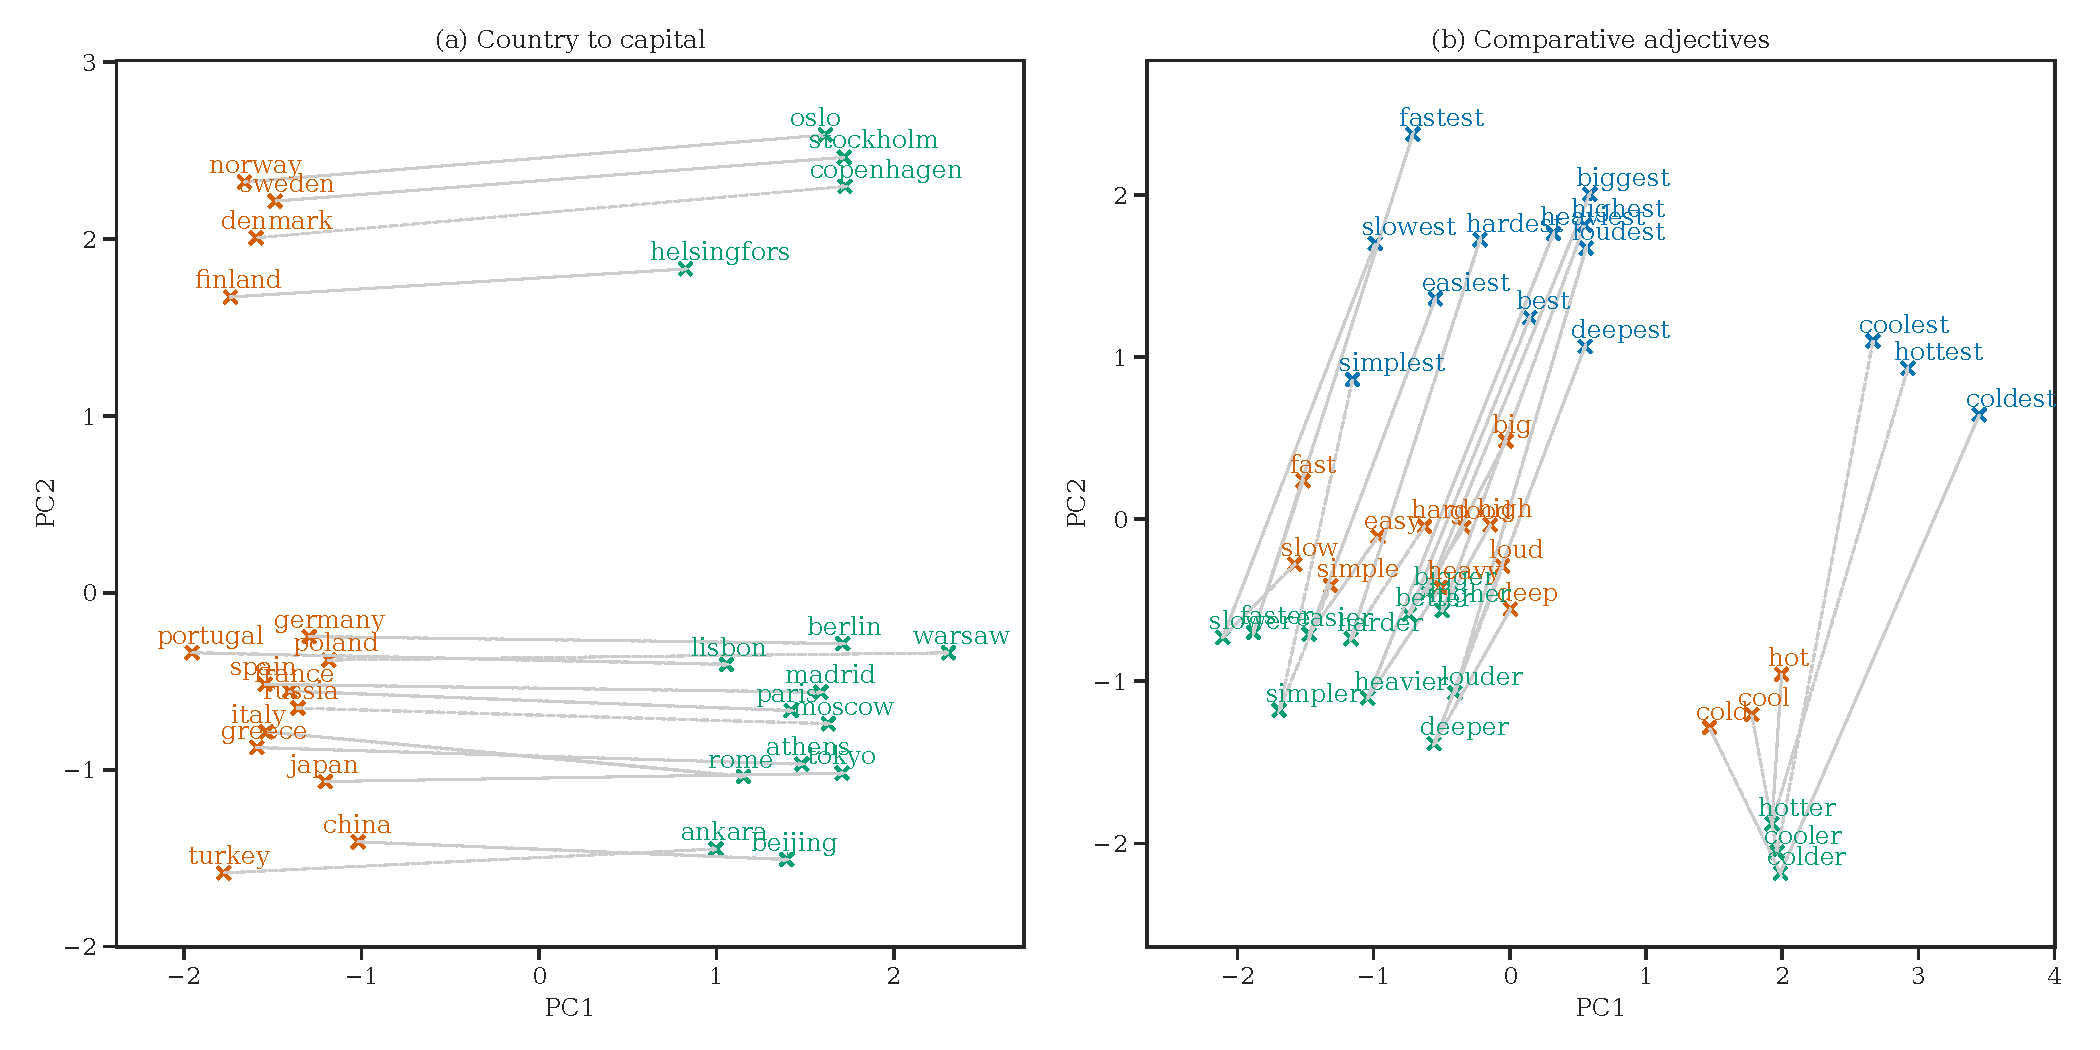
\includegraphics[width=\textwidth]{thesis/figures/word-to-word-relationships-pca-2d.pdf}
 \caption{2-dimensional PCA embeddings of the word embeddings of the SGNS-enwiki model. The plots show how the SGNS-enwiki model understands concepts such as countries and their capital cities (a), as well as and comparative adjectives (b). This figure is inspired by \cite[Figure 2]{mikolov2013b}.}
 \label{fig:sgns-enwiki-word-to-word-relations-pca-2d}
\end{figure}

Next, we will further investigate the notion of clustering, partially motivated by the results we see in \cref{fig:sgns-enwiki-word-to-word-relations-pca-2d}. In particular, to deepen our understanding of the underlying structure of the SGNS-model, we will in the next section perform cluster analysis of its word embeddings. We will use multiple clustering algorithms and internal cluster validation methods to find the most suitable clustering algorithm and hyperparameters.